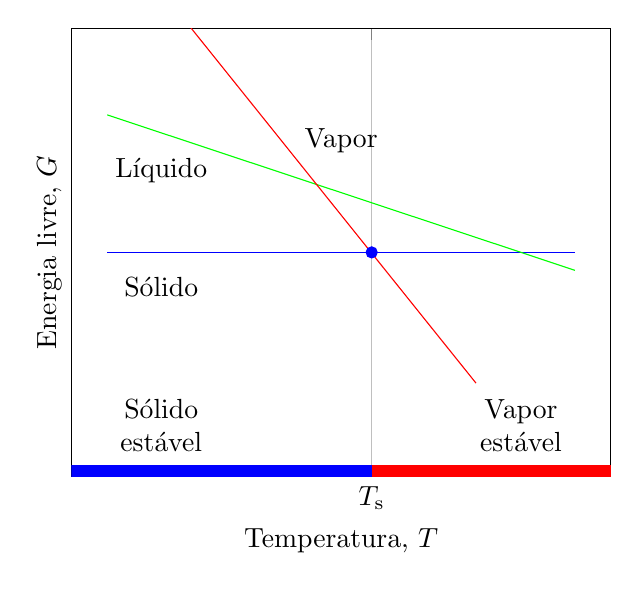
\begin{tikzpicture}
    \begin{axis}
        [
            grid = major,
            ylabel = {Energia livre, $G$},
            xlabel = {Temperatura, $T$},
            domain = 0.2:2.8,
            xmin = 0, xmax = 3,
            ymin = -15, ymax = 15,
            xtick= {1.67}, 
            xticklabels={$T_\mathrm{s}$},
            ytick=\empty,
        ]
        \addplot [ blue ]
            { 0 };
 
         \addplot [ green ]
            { 5-4*x + 5 };
 
        \addplot [ red, domain=0:2.25 ]
            { 25-15*x };
 
         \addplot [ mark=*, color=blue, only marks ] coordinates
             { (1.67, 0) };
 
         \addplot [ blue, line width = 2ex, domain = 0:1.67 ]
             { -15 };
     
         \addplot [red, line width = 2ex, domain = 1.67:3]
             { -15 };
 
         \node [anchor = south, align=center] at (axis cs:0.5, -14) 
             { Sólido\\estável };
 
         \node [anchor = south, align=center] at (axis cs:2.5, -14) 
             { Vapor\\estável };
 
         \node [anchor = north] at (axis cs:0.5, -1) 
             { Sólido };
 
         \node [anchor = south] at (axis cs:0.5, 4) 
             { Líquido };
 
         \node [anchor = south] at (axis cs:1.5, 6) 
             { Vapor };
 \end{axis}
 \end{tikzpicture}